\newpage
\section{Einführung}

% ------------------------------------------------------------------------------
\subsection{Vektorbegriff}

Vektoren sind eine neues Grundelement der Mathematik, welche die Zahlen ergänzen. Im Gegensatz zu Zahlen besitzen Vektoren auch eine \textbf{Richtung}.

Ein Vektor kann als Verschiebung interpretiert werden.

% ------------------------------------------------------------------------------
\subsection{Darstellung}

Ein Vektor $\vv{a}$ wird als Pfeil dargestellt und mit einem Kleinbuchstaben mit Pfeil beschriftet.
\begin{center}
  \begin{tikzpicture}
    \tkzDefPoint(0,0){A1}
    \tkzDefShiftPoint[A1](3,0.8){A2}
    \tkzDrawSegment[thick,-LaTeX](A1,A2)
    \tkzLabelSegment[above left](A1,A2){$\vv{a}$}
  \end{tikzpicture}
\end{center}

% ------------------------------------------------------------------------------
\subsection{Definition durch Endpunkte}

Ein Vektor $\vv{a}$ kann durch einen Anfangspunkt $A$ und einen Endpunkt $B$ definiert werden. Dazu wird die folgende Schreibweise verwendet:
\[
  \vv{a} = \vv{AB}
\]
\begin{center}
  \begin{tikzpicture}
    \tkzDefPoint(0,0){A}
    \tkzDefShiftPoint[A](3,0.8){B}
    \tkzDrawSegment[thick,-LaTeX](A,B)
    \tkzLabelSegment[above left](A,B){$\vv{a}$}
    \tkzDrawPoints(A,B)
    \tkzLabelPoints[left](A)
    \tkzLabelPoints[right](B)
  \end{tikzpicture}
\end{center}
Da der Vektor gerichtet ist, ist die Reihenfolge der Punkte wichtig. Der Vektor $\vv{BA}$ ist ein anderer Vektor als $\vv{AB}$.

\newpage
% ------------------------------------------------------------------------------
\subsection{Addition}

Die Addition von Vektoren ist die Aneinanderreihung von Verschiebungen. Wird ein Punkt $A$ zunächst um den Vektor $\vv{a}$ verschoben und anschliessend um den Vektor $\vv{b}$, so kommt der Punkt bei $C$ zu liegen. Die gleiche Verschiebung entsteht, wenn der Punkt $A$ um den Vektor
\[
  \vv{c} = \vv{a} + \vv{b}
\]
verschoben wird:
\begin{center}
  \begin{tikzpicture}
    \tkzDefPoint(0,0){A}
    \tkzDefShiftPoint[A](2,2){D}
    \tkzDefShiftPoint[D](4,-1){C}
    \tkzDrawPoints(A,C)
    \tkzLabelPoints[left](A)
    \tkzLabelPoints[right](C)

    \tkzDrawSegment[thick,-LaTeX](A,D)
    \tkzLabelSegment[above left](A,D){$\vv{a}$}

    \tkzDrawSegment[thick,-LaTeX](D,C)
    \tkzLabelSegment[above right](D,C){$\vv{b}$}

    \tkzDrawSegment[red,thick,-LaTeX](A,C)
    \tkzLabelSegment[red,above left](A,C){$\vv{c}$}
  \end{tikzpicture}
\end{center}

Die Addition von Vektoren ist \textbf{kommutativ}. Es spielt keine Rolle, ob der Vektor $\vv{b}$ an den Vektor $\vv{a}$ angehängt wird oder umgekehrt. Als Summe entsteht in beiden Fällen der gleiche Vektor $\vv{c}$. Die beiden Varianten der Addition bilden ein Parallelogramm.
\[
  \vv{c} = \vv{a} + \vv{b} = \vv{b} + \vv{a}
\]
\begin{center}
  \begin{tikzpicture}
    \tkzDefPoint(0,0){A}
    \tkzDefShiftPoint[A](2,2){D}
    \tkzDefShiftPoint[D](4,-1){C}
    \tkzDefShiftPoint[A](4,-1){B}
    \tkzDrawPoints(A,C)
    \tkzLabelPoints[left](A)
    \tkzLabelPoints[right](C)

    \tkzDrawSegment[thick,-LaTeX](A,B)
    \tkzLabelSegment[below left](A,B){$\vv{a}$}

    \tkzDrawSegment[thick,-LaTeX](B,C)
    \tkzLabelSegment[below right](B,C){$\vv{a}$}

    \tkzDrawSegment[thick,-LaTeX](A,D)
    \tkzLabelSegment[above left](A,D){$\vv{b}$}

    \tkzDrawSegment[thick,-LaTeX](D,C)
    \tkzLabelSegment[above right](D,C){$\vv{b}$}

    \tkzDrawSegment[red,thick,-LaTeX](A,C)
    \tkzLabelSegment[red,above left](A,C){$\vv{c}$}
  \end{tikzpicture}
\end{center}

% ------------------------------------------------------------------------------
\subsection{Skalierung}
Wird ein Vektor $\vv{a}$ zu sich selbst addiert, so entsteht ein paralleler Vektor zu $\vv{a}$ mit doppelter Länge. Der Vektor wird also zwei Mal genommen, geschrieben:
\[
  \vv{a} + \vv{a} = 2\cdot\vv{a} = 2\vv{a}
\]
\begin{center}
  \begin{tikzpicture}
    \tkzDefPoint(0,0){A1}
    \tkzDefShiftPoint[A1](3,0.8){A2}
    \tkzDefShiftPoint[A2](3,0.8){A3}
    \tkzDefShiftPoint[A1](0.1,-0.3){B1}
    \tkzDefShiftPoint[A3](0.1,-0.3){B2}
    \tkzDrawSegment[thick,-LaTeX](A1,A2)
    \tkzLabelSegment[above left](A1,A2){$\vv{a}$}

    \tkzDrawSegment[thick,-LaTeX](A2,A3)
    \tkzLabelSegment[above left](A2,A3){$\vv{a}$}

    \tkzDrawSegment[thick,red,-LaTeX](B1,B2)
    \tkzLabelSegment[red,below right](B1,B2){$2\vv{a}$}
  \end{tikzpicture}
\end{center}
Allgemein kann das mehrfache Addieren des gleichen Vektors als Multiplikation mit einer natürlichen Zahl geschrieben werden:
\[
  n\cdot\vv{a} = n\vv{a} := \underbrace{\vv{a} + \vv{a} + \vv{a} + \cdots + \vv{a}}_{n-\text{mal}}
\]


% ------------------------------------------------------------------------------
\subsection{Gegenvektor}

Der Gegenvektor eines Vektors $\vv{a}$ ist der Vektor, der gleich lang ist wie $\vv{a}$ und in die umgekehrte Richtung zeigt. Der Gegenvektor wird mit $-\vv{a}$ bezeichnet.

\begin{center}
  \begin{tikzpicture}
    \tkzDefPoint(0,0){A1}
    \tkzDefShiftPoint[A1](3,0.8){A2}
    \tkzDefShiftPoint[A1](0.1,-0.3){B2}
    \tkzDefShiftPoint[A2](0.1,-0.3){B1}
    \tkzDrawSegment[thick,-LaTeX](A1,A2)
    \tkzLabelSegment[above left](A1,A2){$\vv{a}$}

    \tkzDrawSegment[thick,red,-LaTeX](B1,B2)
    \tkzLabelSegment[red,below right](B1,B2){$-\vv{a}$}
  \end{tikzpicture}
\end{center}



% ------------------------------------------------------------------------------
\subsection{Subtraktion}

Die Subtraktion von Vektoren kann auf zwei Arten definiert werden. Erstens kann die Subtraktion eines Vektors $\vv{b}$ vom Vektor $\vv{a}$ als Addition des Gegenvektors $-\vv{b}$ betrachtet werden:
\[
  \vv{c} = \vv{a} - \vv{b} = \vv{a} + \left(-\vv{b}\right)
\]
\begin{center}
  \begin{tikzpicture}
    \tkzDefPoint(0,0){A}
    \tkzDefPoint(2,2){B}
    \tkzDefPoint(-2,3){Z1}
    \tkzDefPoint(6,1){Z}
    \tkzDrawPoints(A,Z)

    \tkzDrawPoint(B)

    \tkzDrawSegment[thick,-LaTeX](A,B)
    \tkzLabelSegment[above left](A,B){$\vv{a}$}

    \tkzDrawSegment[thick,-LaTeX](B,Z1)
    \tkzLabelSegment[above right](B,Z1){$-\vv{b}$}

    \tkzDrawSegment[thick,-LaTeX](B,Z)
    \tkzLabelSegment[above right](B,Z){$\vv{b}$}

    \tkzDrawSegment[red,thick,-LaTeX](A,Z1)
    \tkzLabelSegment[red,below left](A,Z1){$\vv{c}$}
  \end{tikzpicture}
\end{center}

Zweitens kann die Subtraktionsgleichung durch addieren von $\vv{b}$ zu einer Addition umgeformt werden:
\[
  \vv{c} = \vv{a} - \vv{b} \qquad\Rightarrow\qquad \vv{c} + \vv{b} = \vv{a}
\]
\begin{center}
  \begin{tikzpicture}
    \tkzDefPoint(0,0){A}
    \tkzDefPoint(2,2){B}
    \tkzDefPoint(-2,3){Z1}

    \tkzDrawSegment[thick,-LaTeX](A,B)
    \tkzLabelSegment[above left](A,B){$\vv{a}$}

    \tkzDrawSegment[thick,-LaTeX](Z1,B)
    \tkzLabelSegment[above right](Z1,B){$\vv{b}$}

    \tkzDrawSegment[red,thick,-LaTeX](A,Z1)
    \tkzLabelSegment[red,below left](A,Z1){$\vv{c}$}
  \end{tikzpicture}
\end{center}
